\setchapterpreamble[u]{\margintoc}
\chapter{Networking and SSH}
\labch{ssh}


\section{Networking}

\subsection{What is networking?}

Have you ever tried to get some work done on a computer
while the internet was down? It's a nightmare.
Modern day computing relies highly on networking.
But what is networking?

\begin{definition}[Networking]
A computer network comprises two or more computers
that are connected—either by cables (wired) or wifi
(wireless)—with the purpose of transmitting, exchanging,
or sharing data and resources.
\end{definition}

We have been using the computer, and linux, for a while now
but the utility of a computer increases exponentially when
it is connected to a network. It allows computers to share
files and resources, and to communicate with each other.
Current day world wide web is built on the internet.

\begin{definition}[Internet]
Internet is a global network of networks that connects
millions of computers worldwide. It allows computers to
connect to other computers across the world through a
hierarchy of routers and servers.
\end{definition}

Learning about networking and how networking works
is useful, although we won't be devling into details
in this book. It is left as an exercise for the reader
to explore external resources if they are interested.

\marginnote{
One succinct blogpost explaining how the internet works
from which the figure \reffig{networks} is taken
is available at
\url{https://www.highspeedinternet.com/resources/how-the-internet-works}
}

\subsection{Types of Networks}

\begin{marginfigure}
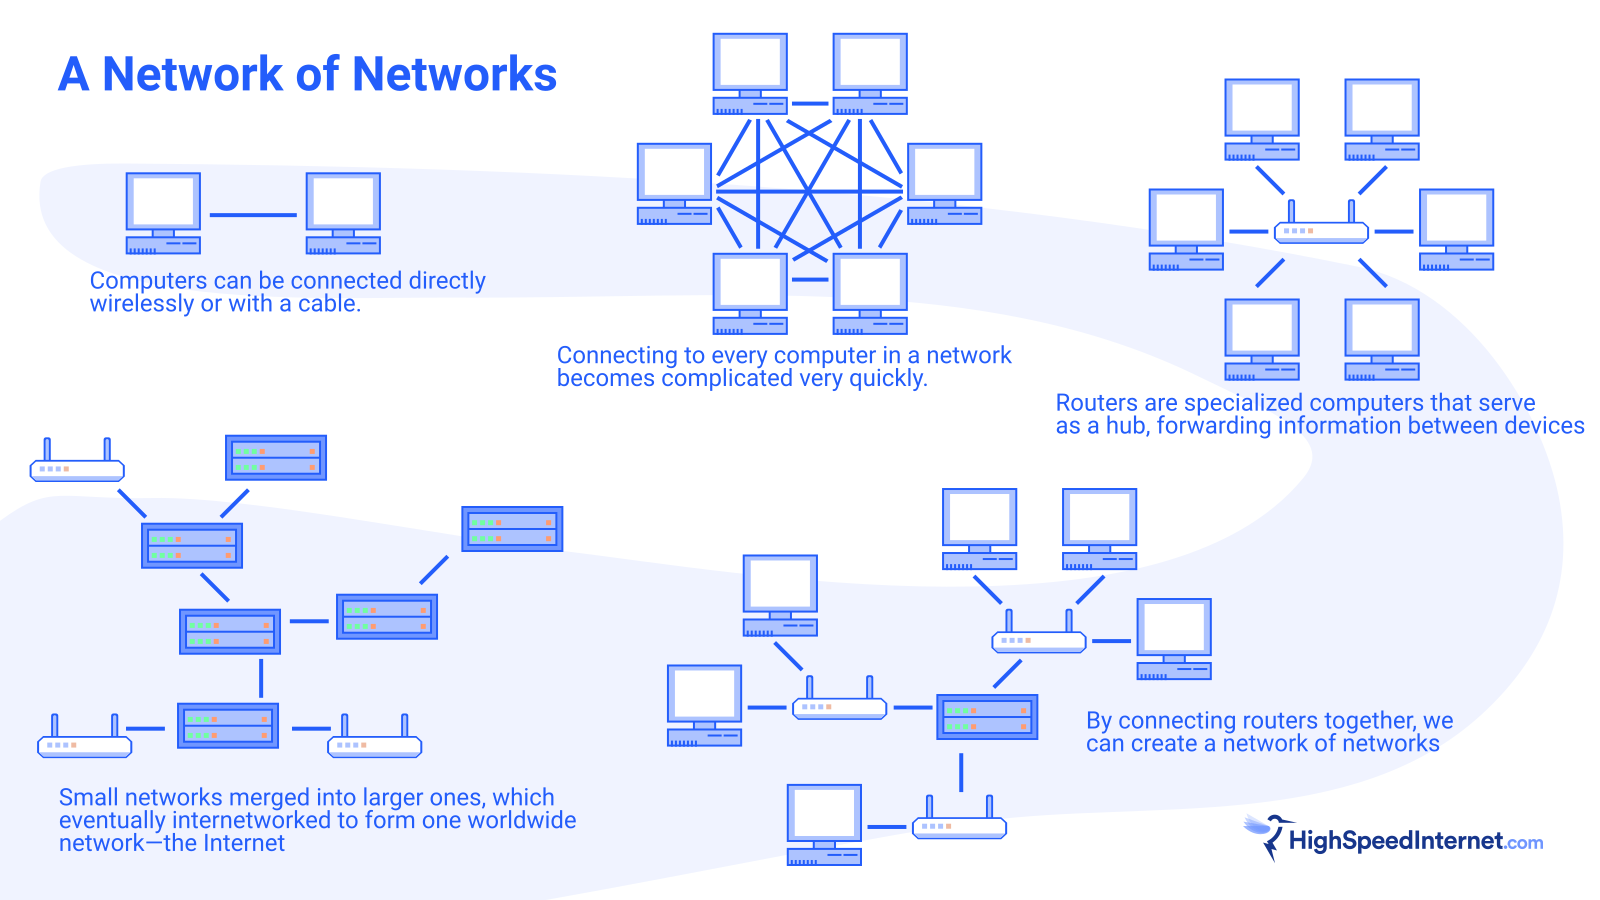
\includegraphics{networks}
\caption{Types of Networks}
\labfig{networks}
\end{marginfigure}

If the end goal is to connect computers with each other,
one naive solution might be to connect all the computers
with each other. Although this might seem intuitive at
first, this quickly gets out of hand when the number of
computers keep increasing.

If we have $n$ computers, then the number of connections
required to connect all the computers with each other
is given by the formula

\[
\frac{n(n-1)}{2} = \frac{n^2 - n}{2}
\]

This is a quadratic function and grows very quickly.

\begin{marginfigure}
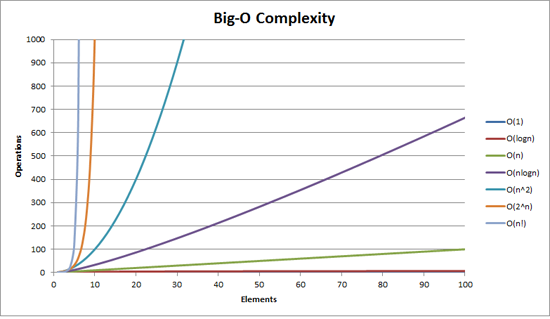
\includegraphics{complexity}
\caption{Growth Rate of Different Functions - Note how quickly $n^2$ grows}
\labfig{complexity}
\end{marginfigure}

This means it will cost a lot to connect all the computers
to each other. This is applicable not only in computer
networking with physical wires, but in many other fields.
Take an examples of airlines and airplane routes. If there
were $n$ airports, then the number of routes required to
connect all the airports is given by the same formula.
This would be disastrous for the economy and the environment
if we ran so many airplanes daily. So what gives?

\textbf{Hub and Spoke Network}

\begin{marginfigure}
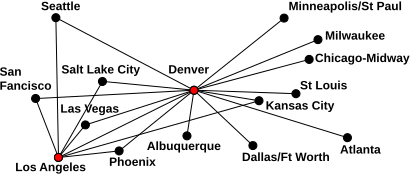
\includegraphics{airlines}
\caption{Hub and Spoke Model Employed by Airlines}
\labfig{airlines}
\end{marginfigure}

The solution to this problem is to use a hub and spoke
model, where there are one, or multiple, central hubs
which connect to many other nodes. Any path from any
node to another goes through one or more hubs. This
reduces the number of connections required to connect
all the nodes.

This is the solution used in airlines, and also in
most computer networks.
\sidenote{
  Although computer networks use a hub model
  for the local area network, the network of
  networks, especially the gateway routers
  follow a mesh model to ensure redundancy
  and make the network more robust.
}

Due to this, networks can be classified into three
broad categories based on their geographical area
coverage.

\begin{marginfigure}
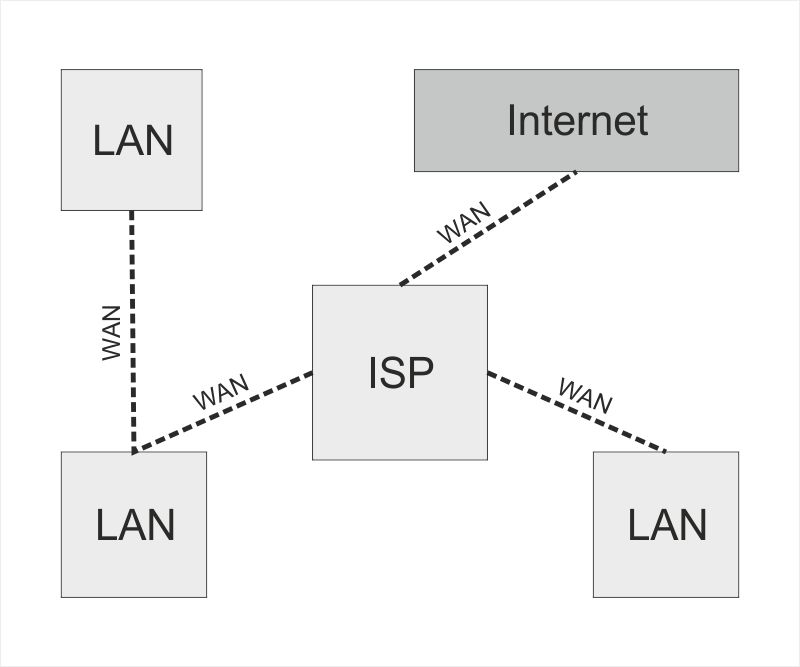
\includegraphics{wan}
\caption{LAN and WAN connecting to the Internet}
\labfig{wan}
\end{marginfigure}

\begin{itemize}
\item \textbf{Local Area Network (LAN)}: A network
that covers a small geographical area, like a
home, office, or a building.
\item \textbf{Metropolitan Area Network (MAN)}:
A network that covers a larger geographical area,
like a city or a town.
\item \textbf{Wide Area Network (WAN)}: A network
that covers a large geographical area, like a
country or the entire world.
\end{itemize}

To connect these networks to computers and also
to each other, we require some special devices.

\subsection{Devices in a Network}

In computer networks, this hub of the
Hub and Spoke Model can either be a
level 1 hub, a level 2 switch, or a level 3 router.

\textbf{Hub}

A hub will simply broadcast the message to all
the connected nodes. This causes a lot of traffic
to be generated and is not very efficient. Hub does
not have the capability to identify which node
is who. This is called a level 1 hub.
\sidenote{
  To understand more about the levels, refer
  \href{https://en.wikipedia.org/wiki/OSI\_model}{OSI Model}
}

\textbf{Switch}

A switch is smarter than a hub. It can identify
each device connected to it and can send the
packets of data only to the intended recipient.
This is more efficient than a hub. This is called
a level 2 switch since it uses the level 2 of the
OSI model (Data Link Layer) to identify the devices.
This means that the devices are identified by their
MAC addresses.
Using this, you can only communicate with devices
in your local network. This is useful for a home
network or a office network. But we cannot communicate
with the entire world using this, since it doesn't
understand IP addresses.

\textbf{Router}

\begin{marginfigure}
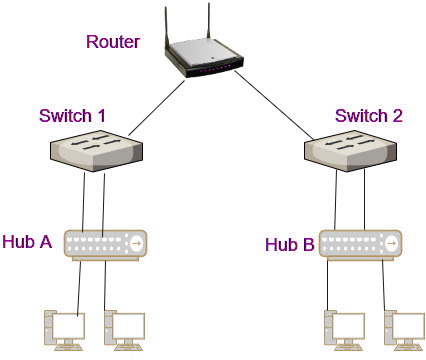
\includegraphics{hsr}
\caption{Hub, Switch, Router connecting to the Internet}
\labfig{hsr}
\end{marginfigure}

A router is even smarter than a switch. It can
understand IP addresses and can route the packets
from one network to another. This is called a level 3
router since it uses the level 3 of the OSI model
(Network Layer) to identify the devices. This means
that the networks are identified by their IP addresses.
This is what we use to connect to the internet.
The internet is nothing but a whole lot of routers
communicating with each other to find the optimal
path to send the packets to its destination.
Border Gateway Protocol (BGP) is the protocol used
by routers to communicate with each other and find
the optimal path. They usually are connected in a
mesh network to ensure redundancy and robustness.

\textbf{Level 3 Switch}

A level 3 switch, or a routing switch, is a switch
with the capabilities of a router. It can understand
the language of IP addresses and can route the packets
to different networks. This is useful in large
organizations where there are many networks and
each network can be divided into subnetworks called
VLANs.

\marginnote{
  You can read more about the differences between
  these devices
  \href{https://www.cbtnuggets.com/blog/technology/networking/l1-l2-vs-l3-whats-the-difference}{online}.
}

So, in short, internet is a network of network
of \dots networks. It is a hierarchical structure
connecting all the computers in the world.
Some computers are connected earlier in the
hierarchy (usually the ones closer geographically)
and some are connected later.

\subsection{IP Addresses}

So how do routers know which where to send the
data packets? This is where IP addresses come in.
To communicate over the internet, two computers
need to know their public IP addresses. The routers
then finds the optimal path to send the data packets
to the destination network.

IP addresses are of two types: IPv4 and IPv6.
The most common one is IPv4, which is a 32-bit
address represented as four octets separated by
dots. For example,

\[
162.136.73.21
\]

Here, each octet can take values from 0 to 255.
\sidenote{
  An octet is a group of 8 bits. Since an IP
  address is 32 bits, it is represented as 4
  groups of 8 bits.
  8 bits can only represent numbers from 0 to 255.
  since $2^8 = 256$.
}
Technically all such combinations are possible
IP addresses, resulting in
$2^{32} = 4,294,967,296$ possible IP addresses.
That is a lot of IP addresses, but not enough
for the growing number of devices in the world.

This is where IPv6 comes in. IPv6 is a 128-bit
address represented as 8 groups of 4 hexadecimal
digits separated by colons. For example,

\[
2001:0db8:85a3:0000:0000:8a2e:0370:7334
\]

\marginnote{
  Notice that there are some groups of zeros
  in the address. These can be compressed by
  writing only one zero in place of multiple
  zeros in each group. Further, any leading
  zeros can be omitted for each group.
  Making the above address as
  \texttt{2001:db8:85a3:0:0:8a2e:370:7334}.
  Further, if there are multiple groups of zeros,
  they can be compressed to \texttt{::}.
  This can be used only once in an address.
  Doing this, the above address can be compressed
  further to
  \texttt{2001:db8:85a3::8a2e:370:7334}.
}

This results in
$2^{128} = 340282366920938463463374607431768211456$
possible IP addresses, which is a lot more than
IPv4.

\subsection{Subnetting and CIDR}

\textbf{Legacy Classes}

\[
10.125.42.62 \rightarrow 0 0 0 0 1 0 1 0 . 0 1 1 1 1 1 0 1 . 0 0 1 0 1 0 1 0 . 0 0 1 1 1 1 1 0
\]

Recall that an IP address, although represented as
four octets, is actually a 32-bit address. This
means that in binary form, an IP address is a
string of 32 1s and 0s. Using the first four bits,
we can classify an IP address into five classes.

\begin{itemize}
\item \textbf{Class A}: The first bit is `0`. The
IP addresses in the range 0.0.0.0 to 127.255.255.255.
\item \textbf{Class B}: The first two bits are `10`.
IP addresses in the range 128.0.0.0 to 191.255.255.255.
\item \textbf{Class C}: The first three bits are `110`.
IP addresses in the range 192.0.0.0 to 223.255.255.255.
\item \textbf{Class D}: The first four bits are `1110`.
IP addresses in the range 224.0.0.0 to 239.255.255.255.
These are reserved for multicast addresses.
\item \textbf{Class E}: The first four bits are `1111`.
IP addresses in the range 240.0.0.0 to 255.255.255.255.
These are reserved for experimental purposes.
\end{itemize}

However, these classes do not simply assign an IP to
each machine. They are further divided into the
network part and the host part.

Class A assigns the first octet to the network part,
this is used to identify which network the machine
is in. The remaining three octets are used to identify
the host in that network. This means that a class A
network can have $2^{24} - 2 = 16,777,214$ hosts.
However, there can only be $2^{7} = 128$ class A
networks. Thus, class A networks are used by large
organizations which have many hosts, but not many
large organizations exist, so 128 networks are enough.

Similarly, class B assigns the first two octets to
identify the network and the remaining two octets
to identify the host. This means that a class B
network can have $2^{16} - 2 = 65,534$ hosts.
And there can be $2^{14} = 16,384$ class B networks.
These are used by medium-sized organizations, which
are plenty in number, and have a moderate number of
hosts.

The same goes for class C networks, where the first
three octets are used to identify the network and
the last octet is used to identify the host. This
network can have $2^{8} - 2 = 254$ hosts. And there
can be $2^{21} = 2,097,152$ class C networks. These
are used by small organizations, which are plenty
in number, and have a small number of hosts.

\textbf{Subnet Masks}

\begin{definition}[Subnetting]
The process of dividing a network into smaller network
sections is called subnetting.
\end{definition}

Usually, each network has only one subnet, which
contains all the hosts in that network. However,
the network can be further divided into smaller
subnetworks, each containing a subset of the hosts.
This is useful in large organizations where the
network is divided into departments, and each
department is given a subnetwork.

To indicate which part of the IP address is the
network part and which part is the host part, we
use a subnet mask. A subnet mask is a 32-bit
number where the first $n$ bits are 1s and the
remaining bits are 0s. The number of 1s in the
subnet mask indicates the number of bits used
to identify the network. For example, for the
IP Address \texttt{192.168.0.15}, it can be
written in binary as
\[
1100 0000 - 1010 1000 - 0000 0000 - 0000 1111
\]

As we know, it belongs to the class C network,
where the first three octets are used to identify
the network, and the rest is used to identify the
host. So the default network mask is

\[
1111 1111 - 1111 1111 - 1111 1111 - 0000 0000
\]

or \texttt{255.255.255.0} in decimal.
The network portion of the IP address is
found by taking the bitwise AND
\sidenote{
  The bitwise AND operation is a binary operation
  that takes two equal-length binary representations
  and performs the logical AND operation on each pair
  of corresponding bits. The result in each position
  is 1 if the first bit is 1 and the second bit is 1;
  otherwise, the result is 0.
}
of the IP address and the subnet mask.
This results in the network address
\[
1100 0000 - 1010 1000 - 0000 0000 - 0000 0000
\]
which is \texttt{192.168.0.0} and the host address
is \texttt{0000 1111} which is $15$.

However, if we do not require all the 8 bits in the
host space
\sidenote{
  That is, if we have less than 254 hosts in the
  network.
}
then we can use some of the initial bits of the
host space to identify subnetworks. This is called
subnetting.

For example, the netmask of \texttt{255.255.255.0}
leaves 8 bits for the host space, or $2^8 - 2 = 254$
\sidenote{
  We subtract 2 from the total number of hosts
  to account for the network address and the
  broadcast address, which are the first(0)
  and the last(255) addresses in the network.
}
hosts. If we want to split this network into
two subnets, we can use the MSB of the host space
for representing the subnetworks. This results in
each subnet having $2^7 - 2 = 126$ hosts.

\begin{remark}
Observe that we effectively lost two available addresses
from the total number of hosts in the network.
Earlier we could have $254$ hosts, but now we can
have only $126 \times 2 = 252$ hosts. This is because
each subnet also reserves the first and the last
address for the network address and the broadcast
address.
\end{remark}

To do this, we change the subnet mask to
\[
1111 1111 - 1111 1111 - 1111 1111 - 1000 0000
\]
which can be represented as \texttt{255.255.255.128}.

This gives us two subnets, one with the address range
of \texttt{192.168.0.1} to \texttt{192.168.0.127}, and
another of \texttt{192.168.0.129} to \texttt{192.168.0.255}.

\subsection{Private and Public IP Addresses}

But what if we want to communicate with computers
in our local network? This is where private IP
comes in. Some ranges of IP addresses are reserved
for private networks. These are not routable over
the internet. Each LAN has a private IP address
range, and the router translates these private
addresses to the public IP address when sending
the packets over the internet. The assignment
of these private IP addresses is done by the
DHCP server
\sidenote{
  Dynamic Host Configuration Protocol (DHCP) is
  a network management protocol used on Internet
  Protocol networks whereby a DHCP server dynamically
  assigns an IP address and other network configuration
  parameters to each device on a network so they can
  communicate with other IP networks.
}
in the router.

Each class of networks has a range of IP addresses
that are reserved for private networks.

\begin{table*}[h!]
\caption{Private IP Address Ranges}
\labtab{privateip}
\begin{tabular}{c c c c}
\toprule
Class & Network Bits (CIDR) & Address Range & Number of Addresses \\
\midrule
\textbf{Class A} & 8 & \texttt{10.0.0.0} - \texttt{10.255.255.255} & 16,777,216 \\
\textbf{Class B} & 12 & \texttt{172.16.0.0} - \texttt{172.31.255.255} & 1,048,576 \\
\textbf{Class C} & 16 & \texttt{192.168.0.0} - \texttt{192.168.255.255} & 65,536 \\
\bottomrule
\end{tabular}
\end{table*}

\subsection{CIDR}

However, this practice of subdividing IP addresses
into classes is a legacy concept, and not followed
anymore. Instead, we use CIDR (Classless Inter-Domain
Routing) to announce how many bits are used to identify
the network and how many bits are used to identify the
host.

For example, we could express the idea that the IP address
\texttt{192.168.0.15} is associated with the netmask
\texttt{255.255.255.0} by using the CIDR notation of
\texttt{192.168.0.15/24}. This means that the first
$24$ bits of the IP address given are considered
significant for the network routing.

This is helpful because not all organizations fit
into the tight categorization of the legacy classes.

\subsection{Ports}

Ports usually refer to physical holes in a computer
where you can connect a cable. However, in networking,
ports refer to logical endpoints for communication.



\vfill
\pagebreak
\subsection{Protocols}
\vfill
\pagebreak
\subsection{Firewalls}
\vfill
\pagebreak
\subsection{SELinux}
\vfill
\pagebreak
\subsection{Network Tools}


\vfill
\pagebreak
\section{SSH}
\subsection{What is SSH?}
\vfill
\pagebreak
\subsection{History}
\vfill
\pagebreak
\subsection{How does SSH work?}
\vfill
\pagebreak
\subsection{Key-based Authentication}
\vfill
\pagebreak
\subsection{Configuring your SSH keys}
\vfill
\pagebreak
\subsection{Configuring your SSH config}
\vfill
\pagebreak
\subsection{How to login to a remote server}
\vfill
\pagebreak
\subsection{Call an exorcist, there's a daemon in my computer}
